\documentclass{article}
\usepackage{graphicx} % Required for inserting images
\usepackage [utf8]{ctex}
\usepackage{listings}

\title{Link Prediction实验}
\author{211870287 丁旭}
\date{September 2023}

\begin{document}

\maketitle

\section{论文摘要abstract}
知识图补全旨在解决带缺失三元组扩展K的问题。在本文中,我们提供了一种方法GenKGC,该方法使用预训练的语言模型将知识图补全转换为序列到序列的生成任务。我们进一步引入了关系引导的演示和实体感知的分层解码,以实现更好的表示学习和快速推理。在三个数据集上的实验结果表明,我们的方法可以获得比基线更好或相当的性能,并且与先前使用预训练语言模型的方法相比,可以实现更快的推理速度。我们还发布了一个新的大规模中文知识图谱数据集OpenBG500用于研究目的 
\par CCS的概念 
计算方法→知识表示和推理。
\par 关键字
知识图谱补全;一代;变压器ACM参考格式:

\section{introduction}
\par 知识图(Knowl edge Graphs , KGs )将现 实世界 中的 知识作 为<主语、
谓语 、宾 语>形 式的 事实 三 元组 ,缩 写为(s ,p ,o ),其中s和o表示实体,p表示实体间的关系,这 有利于 广泛的 知识密 集型任务 。
知识图 谱补 全(Knowledge graph completion, KGC )旨在通过 预测缺
失三 元 组来 补全 知 识图 谱 。在 本 文中 ,我 们 主要 基 于强 大 的预训
练语言模型, 针对 KGC 的链接 预测任务 。
\par 大多数以前的 KG 补全方法,如 TransE[2] 、ComplEx[11] 和
RotatE[9],都 是知 识 嵌入 技 术, 它 们将 实 体和 关 系嵌 入 到向 量空
间中 , 然后 通过 对 这些 向 量利 用预 定 义的 评 分函 数 来获 得预 测的
三 元 组 。 最 近 , 已 经 提 出 了 一 些 文 本 编 码 方 法 ( 例 如 KG-BERT[14]),
它 们利 用 预 训 练 的 语言 模 型 对 三 元 组 进行 编 码 ,并输出 每 个候 选对 象 的分 数 。显 然, 之 前的 大 多数 方 法都 利用 了带有预 定 义评 分函 数 的区 分 范式 来进 行 知识 嵌 入。 然 而, 这种 判别
策略 在 推理 中需 要 对所 有 可能 的三 元 组进 行 昂贵 的 评分 ,并 且受
到负抽 样的 不稳 定性 的影 响。 此外 ,那 些密 集的 知识 嵌入 方法(如
TransE)忽略 了实 体和 关系 之 间的 细粒 度交 互, 并且 必须 为 大规模
的现 实 世界 知识 图 分配 大 量的 内存 占 用。 因 此, 为 知识 图补 全寻
找新的技术解 决方 案是很 直观 的。
\par 在本文中,我们首先用序列到序列的生成对知识图补全建模,
并提出了一种新的方法 GenKGC 。具体来说,我们将实体和关
系表示为输入序列,并利用预训练的语言模型来生成目标实体。
遵循 GPT-3 朴 素的 “ 上下文学习 ” 范 式, 其 中 模 型可 以 通 过连
接与输入相关的选定样本来学习正确的输出答案,我们通过添
加相同关系的三元组来提出关系引导演示。此外,在生成过程
中,我们提出了实体感知的分层解码,以降低生成的时间复杂
度 。 在 两 个 数 据集 WN18RR 、FB15k-237 和新发布的大规模中
文 KG 数据 集 OpenBG500 上 的实 验 结果 证明 了 所提 出 方法 的有
效性。我 们的 工作 贡 献如 下:
\par •我 们 将 链 路 预 测 转 换 为 序 列 到 序 列 生 成 , 并 提 出 了
GenKGC ,在保 持性 能的 同时 减少了 推理 时间 。
\par •我 们 提 出 了关 系 导 向 的 演 示 和 实体 感 知 的 分 层 解 码, 可 以
更好地表示实 体和 关系, 降低 生成 的时 间复杂 度。
\par •我 们 报 告 了两 个 数 据 集 的 结 果 ,并 发 布 了 一 个 新 的大 规 模
KG 数据集 OpenB G500, 用于 研究 目的 。
\section{问题描述}
\par 知识图谱将现实世界中的知识形式化为三元组格式:<subject, predicate, object>, 即<s, p, o>。其中s和o表示实体,p表示实体间的关系。知识图谱补齐(KGC)是解决补齐知识图谱中缺失三元组的问题。很多先前知识图谱补齐的方法,例如:TransE、ComplEx、RotatE,都是将实体和关系嵌入到向量空间,并通过在向量上使用预定义的打分函数来获得预测的三元组。近来也出现了一些文本编码方法(如KG- BERT),利用预训练语言模型编码三元组,再为每个候选输出分数。但是该方法需要在推理时为所有可能的三元组打分,因此代价很昂贵,并存在负样本导致的不稳定性问题。这些密集知识嵌入方法都忽略了实体和关系之间的细粒度交互,并不得不为大规模知识图谱分配庞大的内存,因此很有必要为KGC提出新的解决方法。

\par 本文提出了一种新方法--GenKGC,即将知识图谱补齐任务转换为seq2seq的生成任务。具体来说,就是将实体和关系作为输入序列,利用预训练语言模型生成目标实体。为了更好的表示学习和快速推理,本文进一步引入了关系引导示例和实体感知层次解码两个策略。并且,在三个数据集上的实验结果表明,本文的方法能获得比之前使用预训练语言模型更好的性能。为了研究需求,本文也发布了一个新的大规模中文知识图谱数据集OpenBG500。

\section{输入、输出、模型算法描述(附框架图;有多个的挑1个主要实现)}
\begin{figure}[htp]
        \centering
        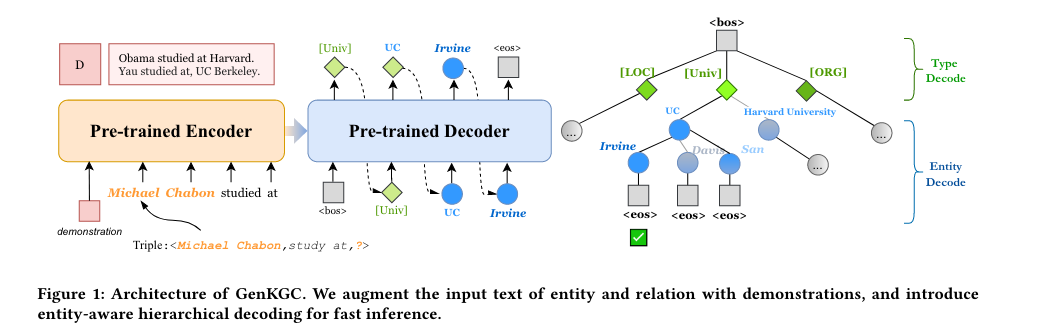
\includegraphics[width=16cm]{框架.png}
        \caption{}
        \label{pic7}
\end{figure}
\par 本论文主要研究了将知识图谱补全任务从判别式方法转化为生成式方法。给定一个不完整的知识图谱三元组集合,任务是预测缺失的实体或关系。

\par 输入: 是一个不完整的知识图谱三元组集合
\par 输出: 是对缺失实体或关系的生成预测。
\par 模型采用了基于生成式Transformer的方法来完成知识图谱补全任务。Link Prediction as Seq2Seq Generation——将链接预测任务形式化为seq2seq的生成任务

\par 知识图谱由实体类别和实体描述定义为:其中是实体集,是关系集,是三元组集,是实体类别,是实体描述。对于每一个 三元组, 分别表示 头、尾实体。同时,对于每个实体 都存在对应的实体类别 和文本描述 。实体链接将补齐知识图谱里缺失三元组当作:在给定头实体和关系的情况下,预测尾实体.

\par 而本文将实体和关系都视为tokens序列,就是用纯文本代替嵌入来表示实体,以此弥补知识图谱中三元组和预训练语言模型之间的差距。具体来说就是,对于给定的缺失尾实体的三元组 ,先分别获得 ,然后将它们拼接起来。如图1所示,将实体描述 "Michael Chabon" 和关系描述 "studies at" 拼接成 "Michael Chabon studies at" 作为输入序列,而输出的目标实体序列就是 "UC, Irvine"。

\par Relation-guided Demonstration关系引导示例

\par受prompt-tuning启发,本文在编码器侧使用关系引导示例 ,以关系 为引导,从训练集中采样一些示例,这些示例包含相同的关系。最后输入序列可以形式化为:
\begin{figure}[htp]
        \centering
        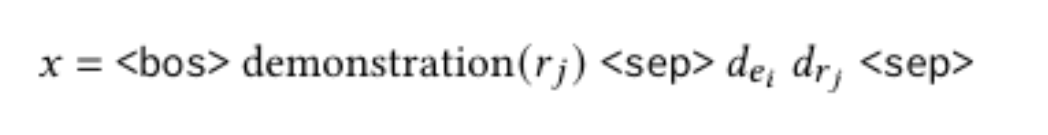
\includegraphics[width=16cm]{序列形式化.png}
        \label{pic7}
\end{figure}

\newpage

\par Entity-aware Hierarchical Decoding
实体感知层次解码
\begin{figure}[htp]
        \centering
        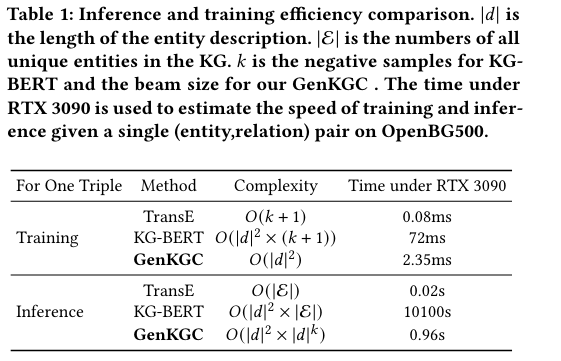
\includegraphics[width=16cm]{1.png}
        \label{pic7}
\end{figure}

\newpage

\par 在平凡解码设定下,需要遍历 中的所有实体,并通过打分函数来排序。但这是非常耗时的,如图1所示。而本文的方法使用波束搜索,从 中取得 top-k 个实体。具体来说,对于 ,GenKGC 通过以下公式计算每个 的分数并排序:

\begin{figure}[htp]
        \centering
        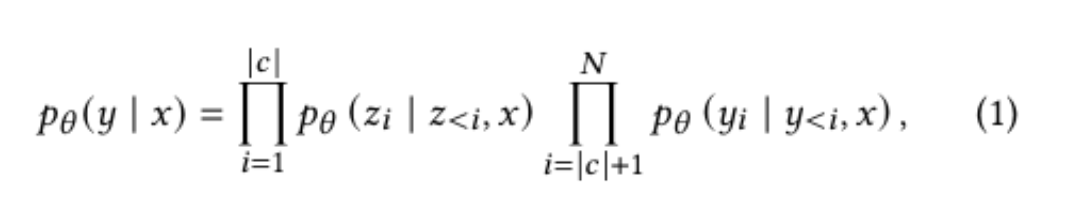
\includegraphics[width=16cm]{2.png}
        \label{pic7}
\end{figure}

\newpage

\par z 是类别 的 个 token 集,y 是文本表示 的 N 个 token 集。
\begin{figure}[htp]
        \centering
        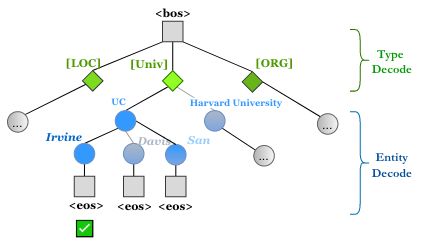
\includegraphics[width=16cm]{3.png}
        \label{pic7}
\end{figure}

\par KG中蕴含着丰富的语义信息,例如实体类型,直觉是对解码进行约束能加速推理。本文在预训练语言模型词汇表中添加一些特殊token来表示类型,以此来约束解码。为确保生成的实体在实体候选集中,本文构建了一颗前缀树,来解码实体名称,具体如图1所示。例如:"UC"后面只能跟随"Irvine"、"Davis"、"San"之一,极大地缩小了解码遍历空间。

类似于普通的seq2seq模型,本文使用标准的seq2seq目标函数来优化GenKGC:
\begin{figure}[htp]
        \centering
        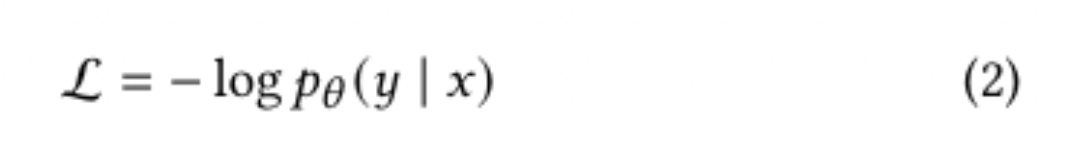
\includegraphics[width=16cm]{4.png}
        \label{pic7}
\end{figure}
\section{评价指标及其计算公式}

本论文采用了以下评价指标对知识图谱补全任务进行评估:

\par Hit@K:

\par "Hit" 表示一个样本是否被正确地命中或预测出来。
"@K" 表示我们关注命中前K个结果的情况。
\par Hit@1:

在测试集上对模型进行评估时,计算每个样本是否在模型的预测结果中命中了正确的答案。
如果某个样本的正确答案是模型的第一个预测结果,那么该样本被认为在 "Hit@1" 下被正确预测。
\par Hit@3:

类似于 "Hit@1",但是在这种情况下,我们关注模型的前三个预测结果。
如果某个样本的正确答案在模型的前三个预测结果中,那么该样本被认为在 "Hit@3" 下被正确预测。
\par Hit@10:

类似于 "Hit@1" 和 "Hit@3",但是在这种情况下,我们关注模型的前十个预测结果。
如果某个样本的正确答案在模型的前十个预测结果中,那么该样本被认为在 "Hit@10" 下被正确预测。
这些指标用于衡量模型对于给定任务的准确性和预测能力。在测试集上进行评估时,通过计算在不同命中率下的准确预测数量,我们可以了解模型的性能表现。具体来说,"Hit@1"、"Hit@3" 和 "Hit@10" 的值越高,表示模型的预测准确率越好。
\section{对比方法及这些对比方法的引用论文出处}
\par 对比结果:

1、GenKGC在所有数据集上都取得了比KG-BERT 更好的结果,并保持着更快的推理速度。

2、TransE等基于转移的方法(将实体、关系视为相同空间中的向量),虽然在一些指标上表现更好,但却面临着内存问题。在OpenBG500上,TransE需要260M的参数来存储所有的实体和关系,而GenKGC使用的预训练语言模型(BART\BERT-base)只需要110M参数。这一问题在实体变得更多时,将更加严重。

\begin{figure}[htp]
        \centering
        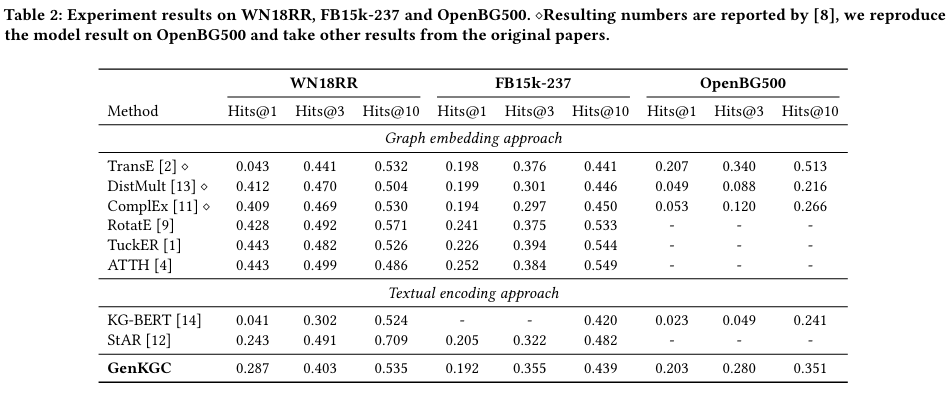
\includegraphics[width=16cm]{模型对比.png}
        \caption{}
        \label{pic7}
\end{figure}
\par 本论文与以下对比方法进行了实验比较,对比方法的引用论文出处如下:
\par TransE:一种常用的基于距离的知识图谱补全模型,它利用欧几里得距离或曼哈顿距离来度量不同实体和关系之间的相似度。
\par
论文:Bordes, A., Usunier, N., Garcia-Duran, A., Weston, J., & Yakhnenko, O. (2013). Translating embeddings for modeling multi-relational data.
\par
ComplEx:一种基于矩阵分解的知识图谱补全模型,它使用复数向量来表示实体和关系,并通过点积运算来计算它们之间的相似度。
\par 论文:Trouillon, T., Welbl, J., Riedel, S., Gaussier, E., & Bouchard, G. (2016). Complex embeddings for simple link prediction.

\par ConvE:使用卷积神经网络(CNN)来学习实体和关系之间的嵌入,然后将它们连接起来以预测缺失的三元组。
\par 论文:Dettmers, T., Minervini, P., Stenetorp, P., & Riedel, S. (2018). Convolutional 2d knowledge graph embeddings.

\par RotatE:一种利用复数旋转来计算实体和关系之间相似度的知识图谱补全模型。
\par 论文:Sun, Z., et al. "Rotate: Knowledge graph embedding by relational rotation in complex space." ICLR 2019.
\section{结果}
\subsection{实验结果}
\begin{enumerate}
    \item 运行代码 ./scripts/openbg.sh
\begin{figure}[htp]
        \centering
        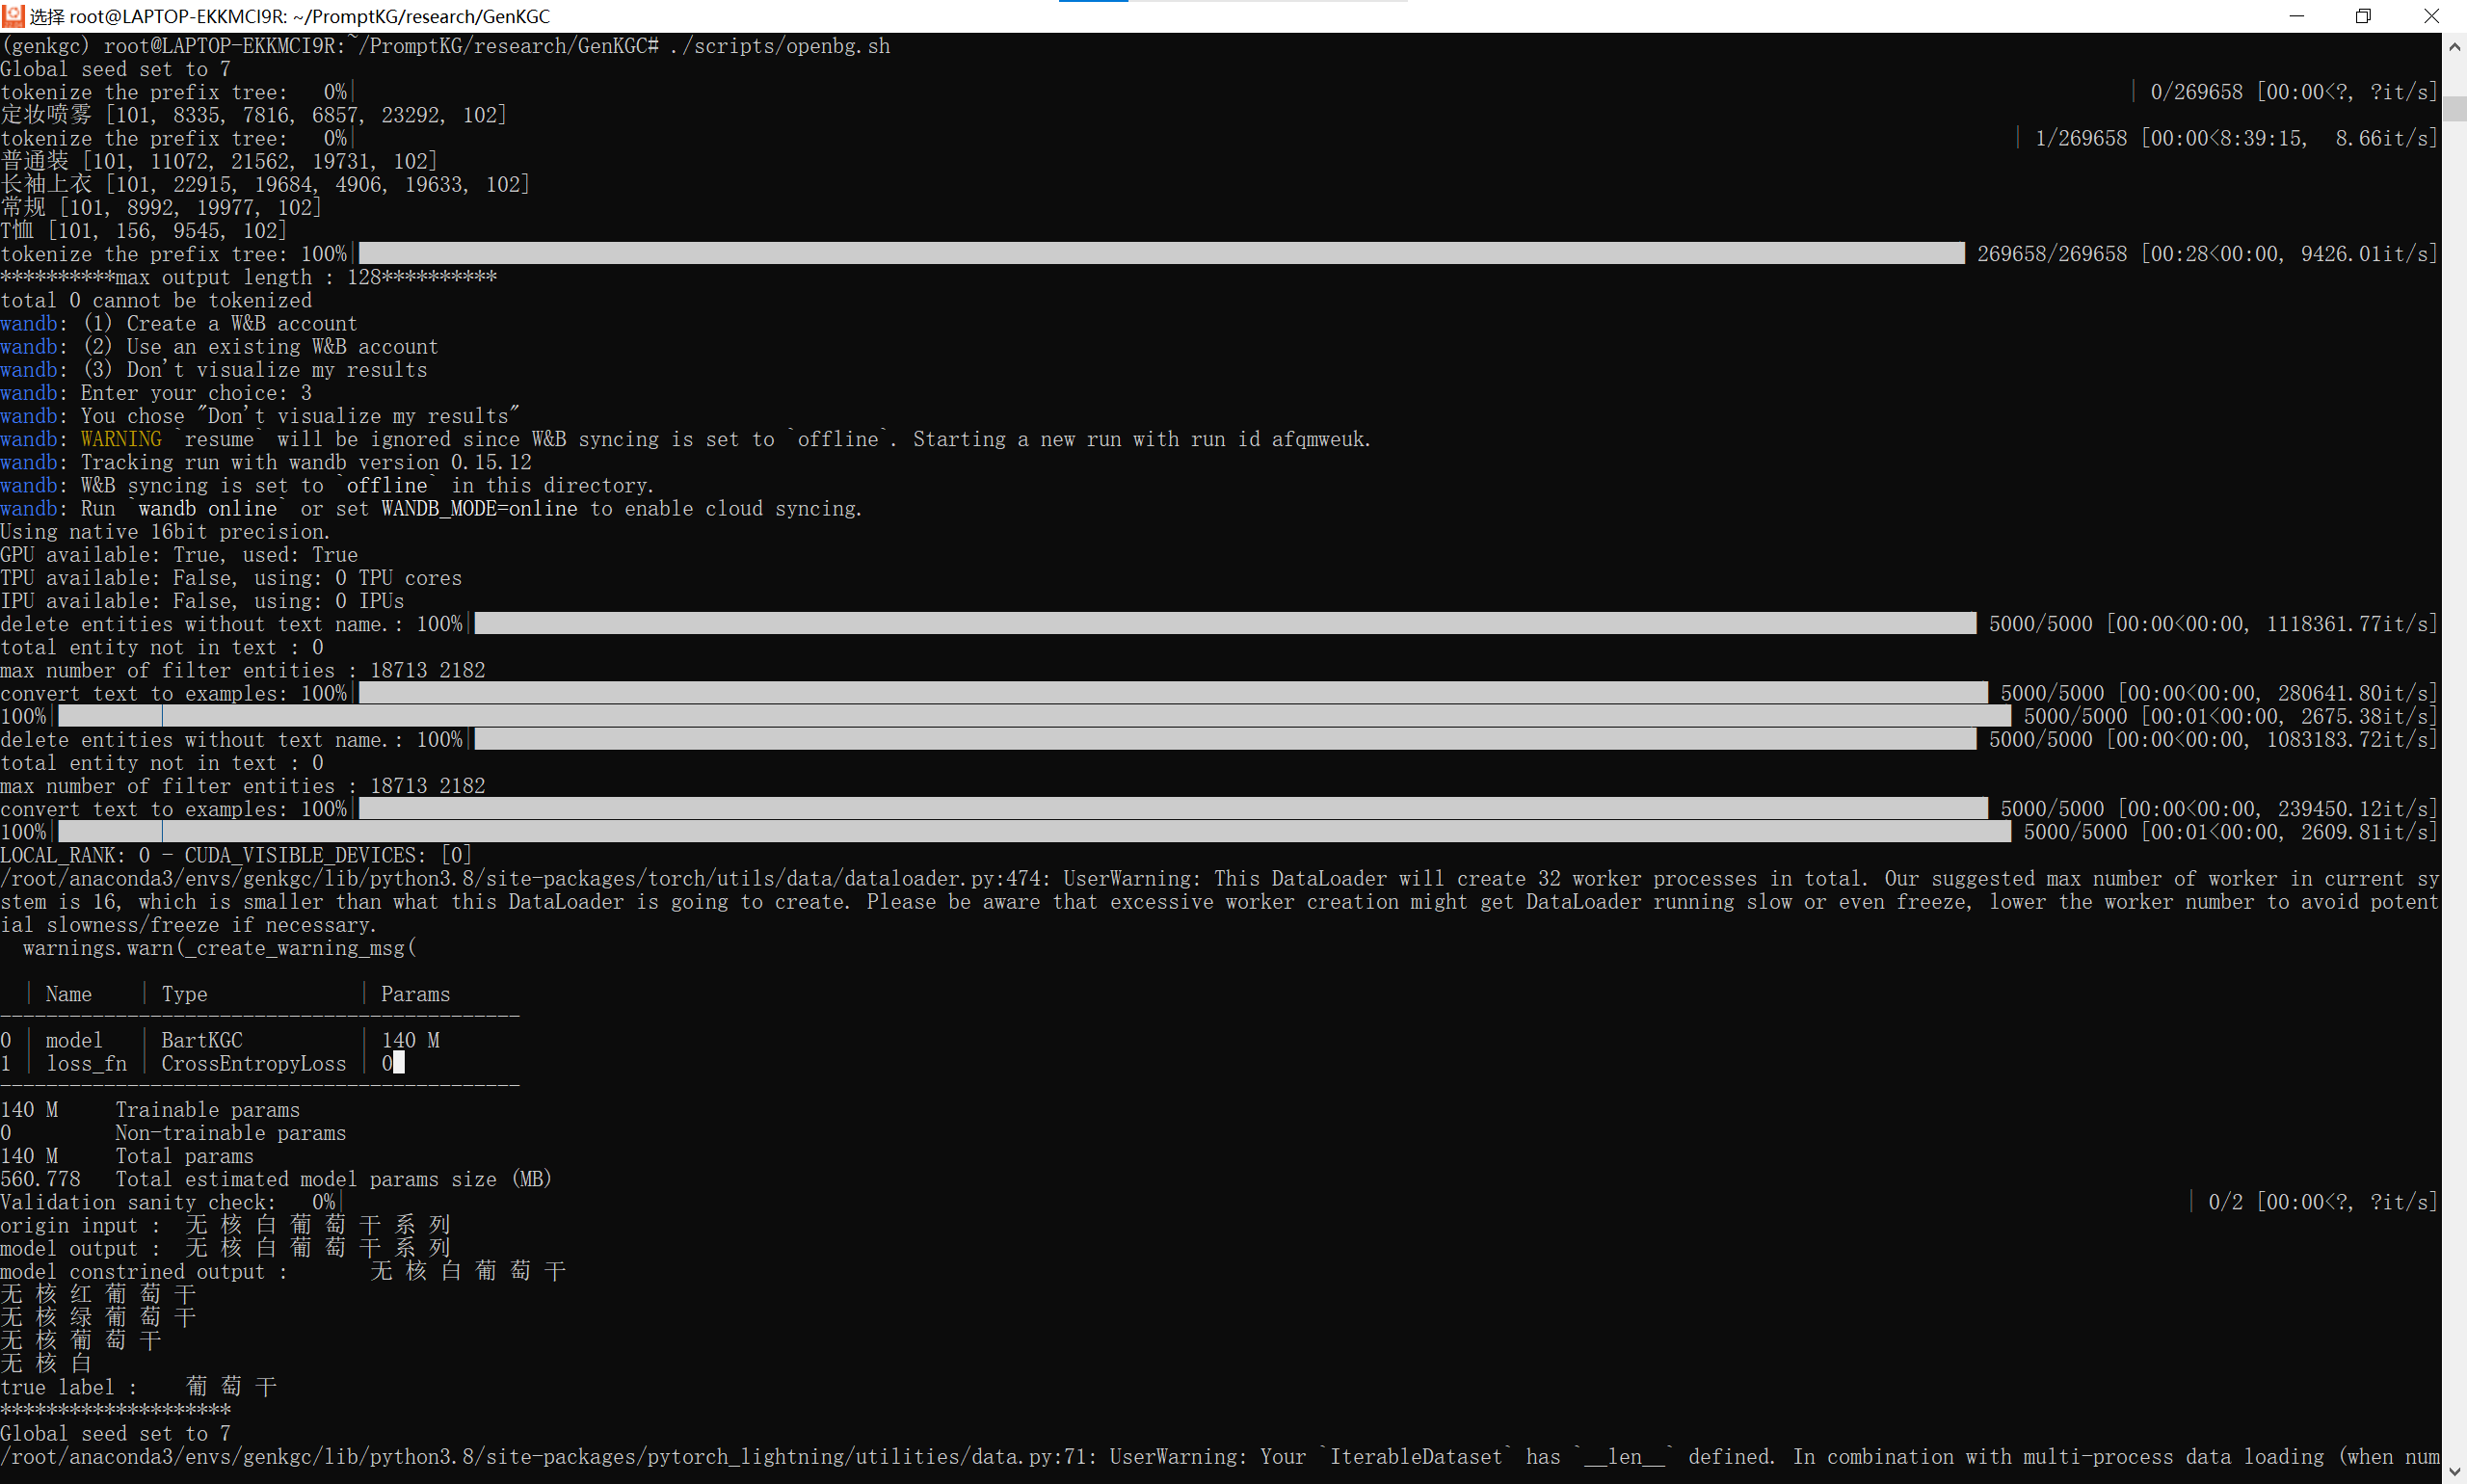
\includegraphics[width=16cm]{run.png}
        \caption{开始运行}
        \label{pic7}
\end{figure}
\begin{figure}[htp]
        \centering
        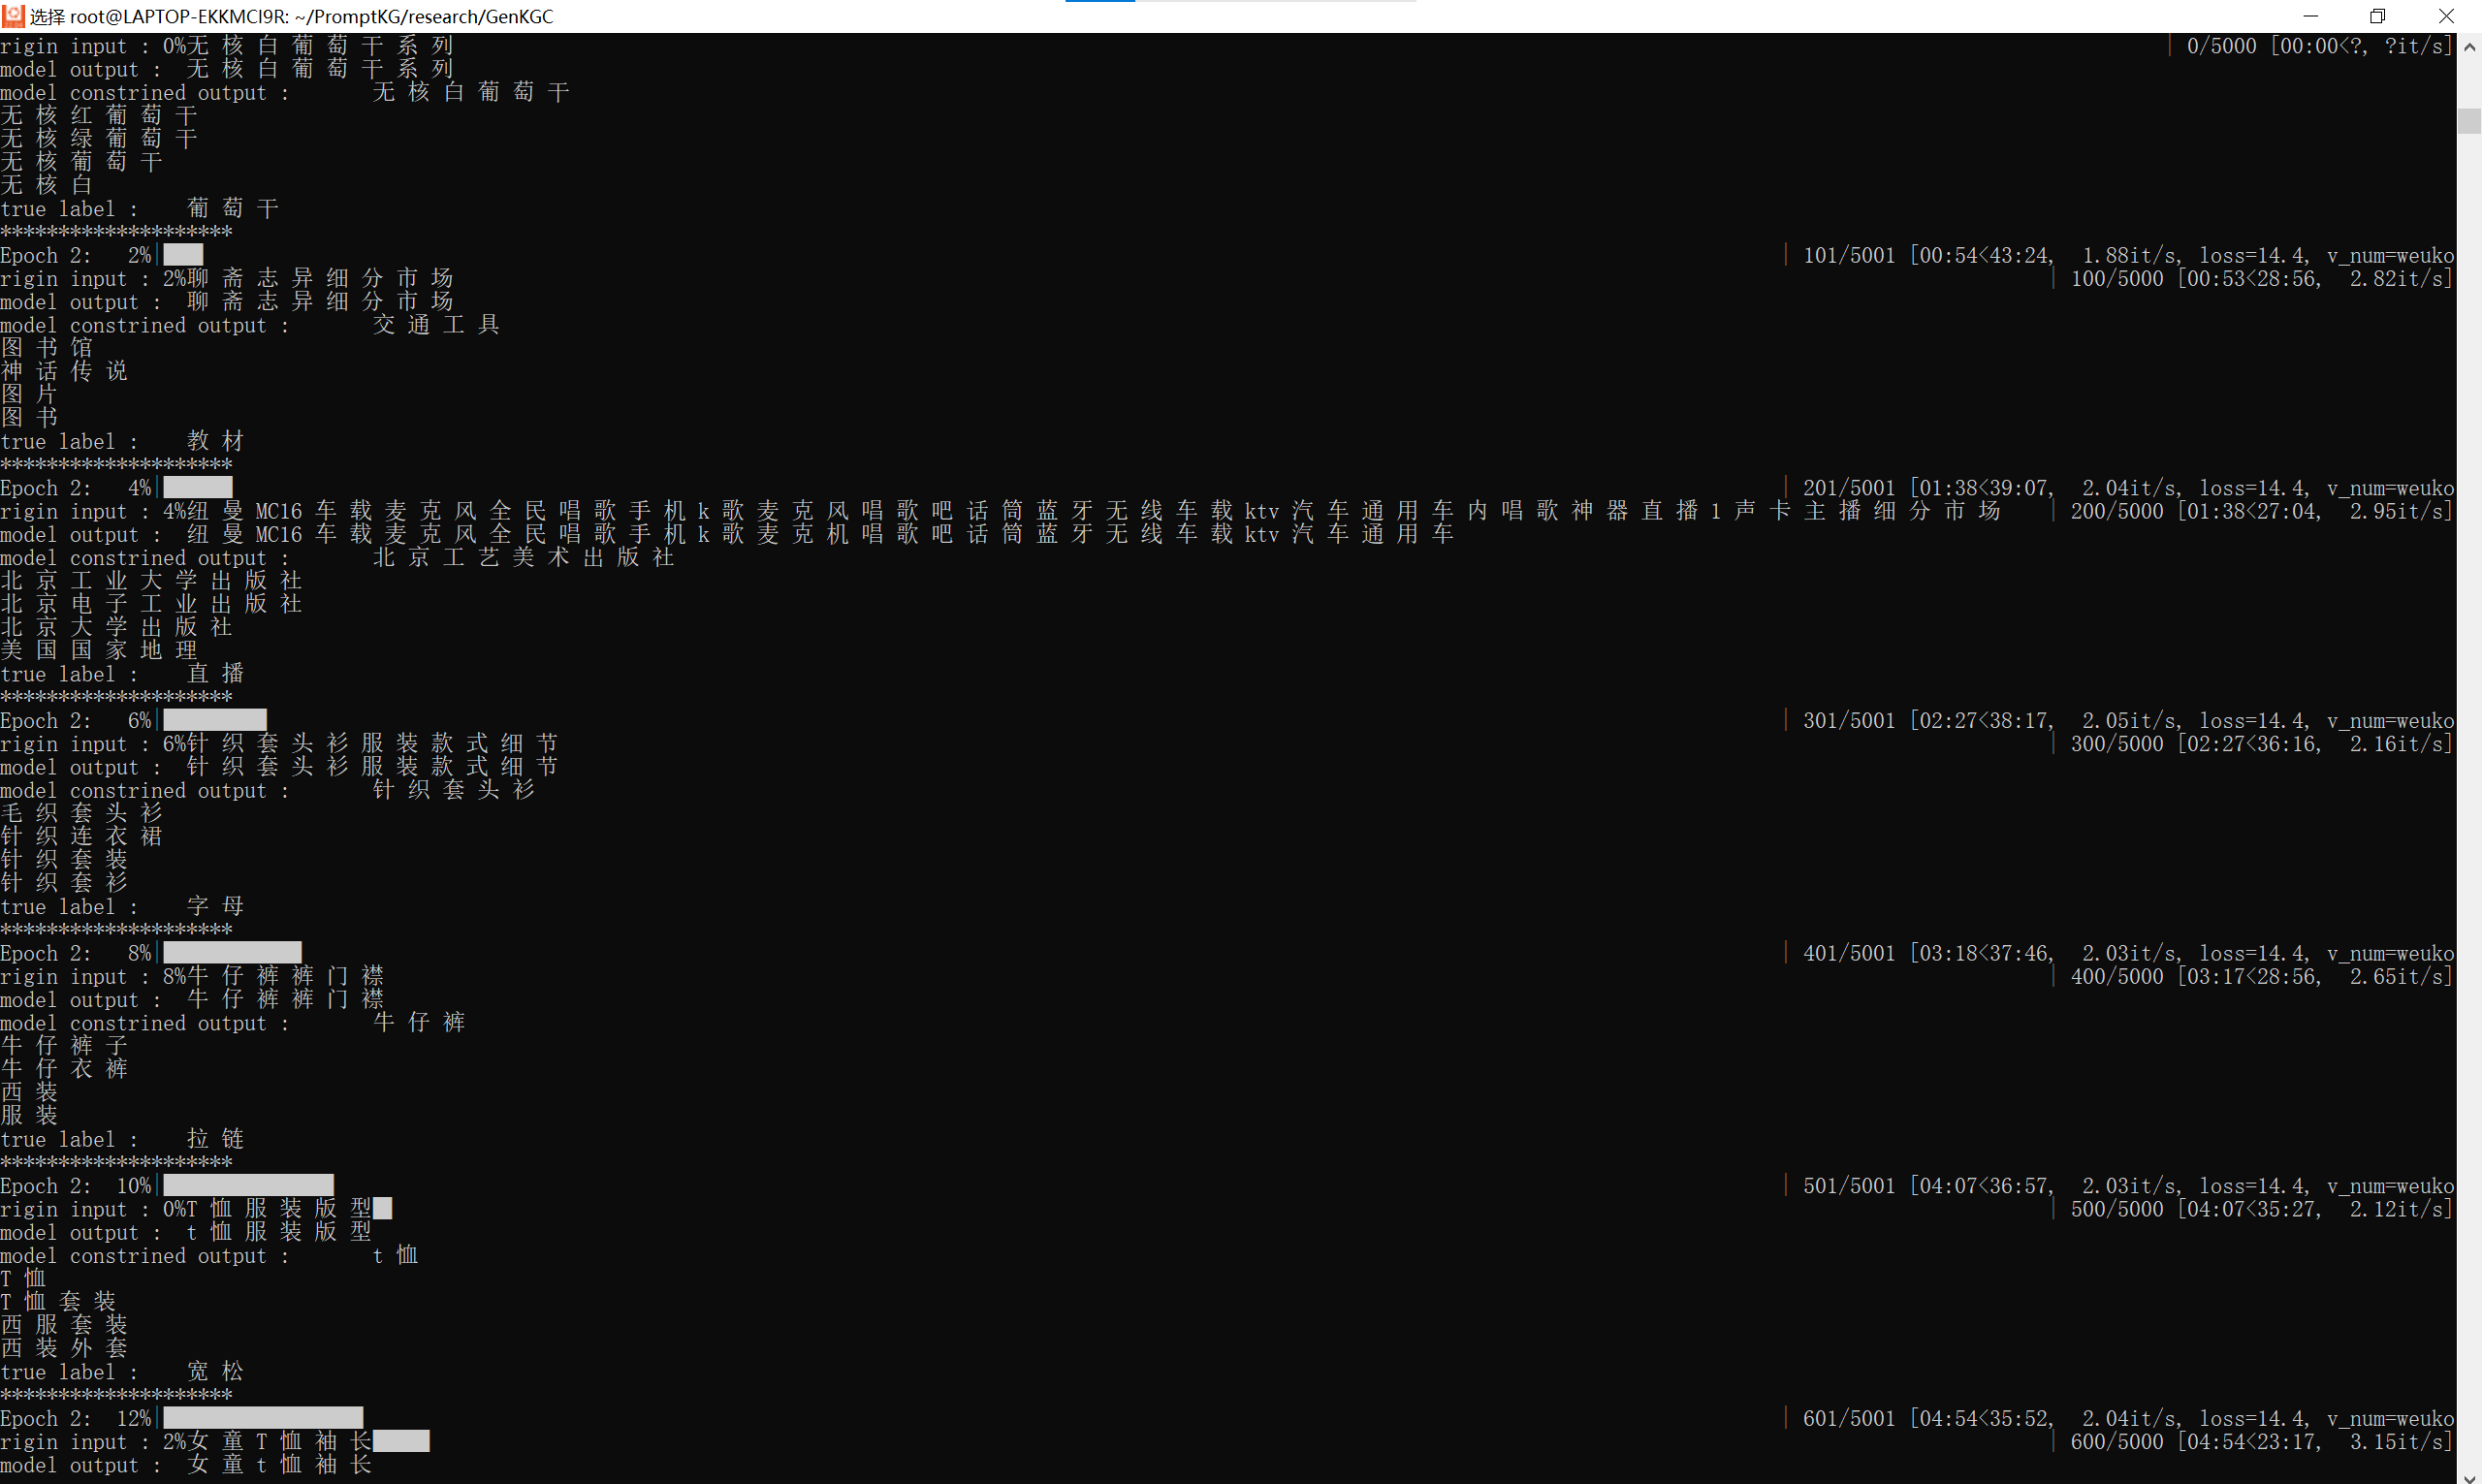
\includegraphics[width=16cm]{过程.png}
        \caption{运行过程}
        \label{pic7}
\end{figure} 
    
    \item 运行结果
    \begin{figure}[htp]
        \centering
        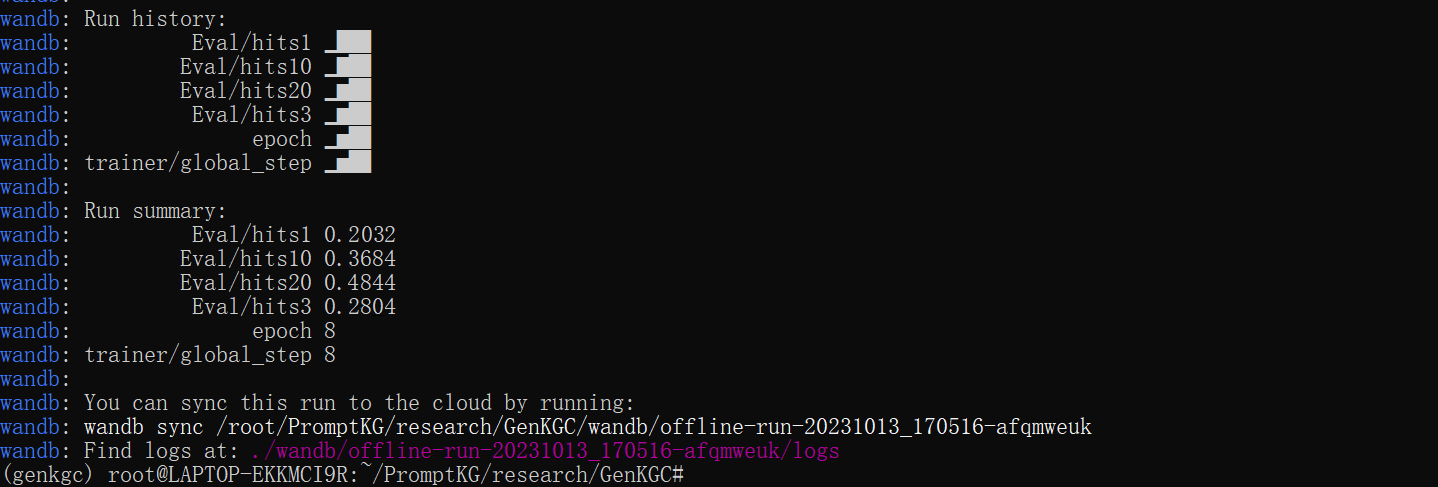
\includegraphics[width=16cm]{最终结果.png}
        \caption{运行结束}
        \label{pic7}    
    \end{figure} 
\end{enumerate}

\newpage

\subsection{论文}
对不同的解码策略分析样例,对于没有使用层次解码的GenKGC,本文使用常规的beam search。从表4可以看出GenKGC生成更好的实体结果,而未使用层次解码的GenKGC更早地停留在正确但不准确的回答上,本文认为这是预训练语言模型自带的偏差造成的。而本文提出的实体层次编码能够约束解码过程并缓解由预训练语言模型带来的偏差。


\begin{figure}[htp]
        \centering
        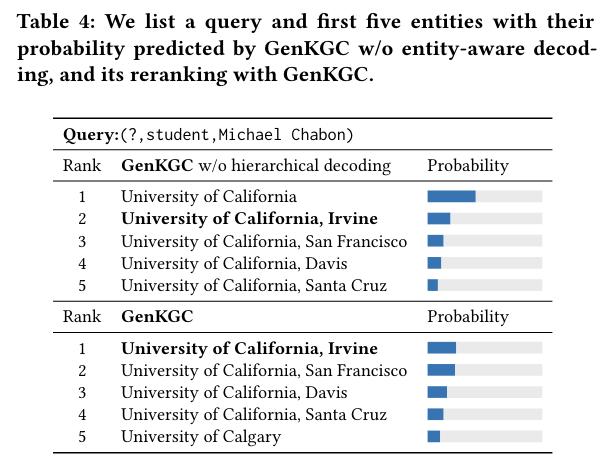
\includegraphics[width=16cm]{结果.png}
        \caption{论文结果}
        \label{pic7}    
    \end{figure} 

\par 在本文 中, GenKGC ,可 以在使 用预 训练 模型 进行
链路 预测 时 达到 可比 较的 结 果, 同时 减 少了 推理 和训 练 成本 。在
三个 基准 数 据集 上的 实验 结 果证 明了 GenKGC的 方法 的有 效 性, 特别
是在推理时 间上。

\end{document}
